%!TEX root = main.tex
\newpage
\section{State of the Art}

Nowadays, people use lot's of services based in cloud and lot's of companies choose to use them too. Using it, companies reduce the costs of IT infrastructure and people don't buy ``physical storage'' and don't care where are the data. The cloud service provide that the data is secure.
But, like any system, the cloud have problems such as another computer systems, software and hardware faults. And the resilience of the cloud is an important characteristic.

The increased use of cloud is related with a low usage of many dedicated servers, lower voltage levels, reduce noise margins and increase clock rates \cite{wolter2012resilience}.

The cloud providers offers resources ready to deliver \cite{wolter2012resilience}.

With this work, I want to inject software faults and analyze how the system react to them.

A lot of studies show that the software faults\cite{avizzienisbasic} it's the main cause of computer failures.

%In this work
%deliberate how

About 44\% of the software faults cannot be emulated \cite{madeira2000emulation}.

% \marginnote{especificar as abreviaturas...}[0cm]
% \ac{cots}
% \ac{g-swfit}
% \ac{odc}
% \ac{swifi}

I had access to the application (executable only, not the source) of Robert Natella, called SAFE, that inject software faults, as I also have to do and I will describe it in next section.

\subsection{SAFE by Robert Natella}
Safe is an application to inject realistic software faults in programs written in C and C++.
This tool uses MCPP as parser, to get the tree of code. The decision of use MCPP instead of GCC parser was a workaround for some of the shortcomings of the GCC's C preprocessor.
After that, write some files, variations of original files (code with simple mutations) with operators applied.
Robert Natella implemented thirteen operators in SAFE, same as João Durães\cite{duraes2006emulation}, but with the difference that Robert implemented at source code level, and João at binary level.

\subsection{ODC Model}
\ac{odc} Model is a framework developed by IBM, created to improve the level of technology available to assist the decisions of a software engineer, via measurement and analysis.
ODC can be used to classifying and analyzing defects during software development.

\red{ essentially a classification of the defects. This model have eight categories:}
\cite{bridge1998orthogonal}
\cite{chillarege2004orthogonal}

\begin{itemize}
	\item \textbf{Function} - This defect affects significant capability, end-user features, product \ac{api}, interface with hardware architecture, or global structure(s). It would require a formal design change.
	\item \textbf{Checking} -
	\item \textbf{Assignment} -
	\item \textbf{Algorithm} -
	\item \textbf{Interface} -
	\item \textbf{Timing/serialization} -
	\item \textbf{Build/package/merge} -
	\item \textbf{Documentation} -
\end{itemize}


\newpage
\section{Research objectives and approach method}

In this section are discussed the main aspects in study.

\subsection{Cloud Computing}

Three levels of Cloud Computing Service Models:

\begin{itemize}
	\item \textbf{\ac{iaas}} - as the name suggests, provides an computing infrastructure, such as virtual machines, firewalls, load balancers, IP addresses, virtual local area networks and others. Examples: Amazon EC2, Windows Azure.

	\item \textbf{\ac{paas}} - provides an computing platform, normally includes operating system, programming language execution environment, database, web server and others. Examples: AWS Elastic Beanstalk, Windows Azure, Heroku.

	\item \textbf{\ac{saas}} - provides access to application softwares ofter referred as \textit{on-demand self-service} sofwares. Use it without install, setup and run the application. Service provider do all things for you. Google Apps, Microsoft Office 365.

\end{itemize}

The cloud computing isn't free of external disturbances\cite{wolter2012resilience}, the most important are:
\begin{itemize}
 	\item Security attacks;
 	\item Accidents;
 	\item Power surges;
 	\item Workload faults;
 	\item Malfunction;
 	\item Worms
 	\item \ac{ddos} attacks.
 \end{itemize}


\subsection{GCC Parser vs Bison vs Eclipse CDT}

In the beginning of planning the basic software without any user interface, I needed to research the best applications, as the best way for using them to obtain panned results (fault injector).
For that, I thought that I can use the same tools that I have used in Compilers course, Lex and Yacc

For parsing the code, analyze and modify it,



Finally I decided to use Eclipse CDT Plugin as standalone (only import libraries to project), because of my facilities in programming in Java Language, the maintainability of software, the low learning level than the developers need to modify it.


\red{Problems with the rewriting of tree}

\red{Reflection}

\red{But I was forced to take decisions after that, for example, after create the tree of code, I can go through the tree in the recursive way or using \textit{Visitor Pattern}.}

\red{Performance analyses}

\subsection{Applications to inject faults}

\red{The same applications that João Durães have collect information?}

\newpage
% \section{Current work and preliminary results}
\section{Fault Injector Development}

\begin{table}[h]
\begin{tabular}{l|l}
\hline
Fault Type & Description                                            \\ \hline
MFC        & Missing function call                                  \\
MVIV       & Missing variable initialization using a value          \\
MVAV       & Missing variable assignment using a value              \\
MVAE       & Missing variable assignment with an expression         \\
MIA        & Missing IF construct around statements                 \\
MIFS       & Missing IF construct + statements                      \\
MIEB       & Missing IF construct + statements + ELSE construct     \\
MLAC       & Missing AND in expression used as branch condition     \\
MLOC       & Missing OR in expression used as branch condition      \\
MLPA       & Missing small and localized part of the algorithm      \\
WVAV       & Wrong value assigned to variable                       \\
WPFV       & Wrong variable used in parameter of function call      \\
WAEP       & Wrong arithmetic expression in function call parameter \\
		   & \red{add another faults}								\\ \hline
\end{tabular}
\caption{\small \sl Faults.\label{tab:faults}}
\end{table}

\begin{table}[ht]
\begin{tabular}{c}
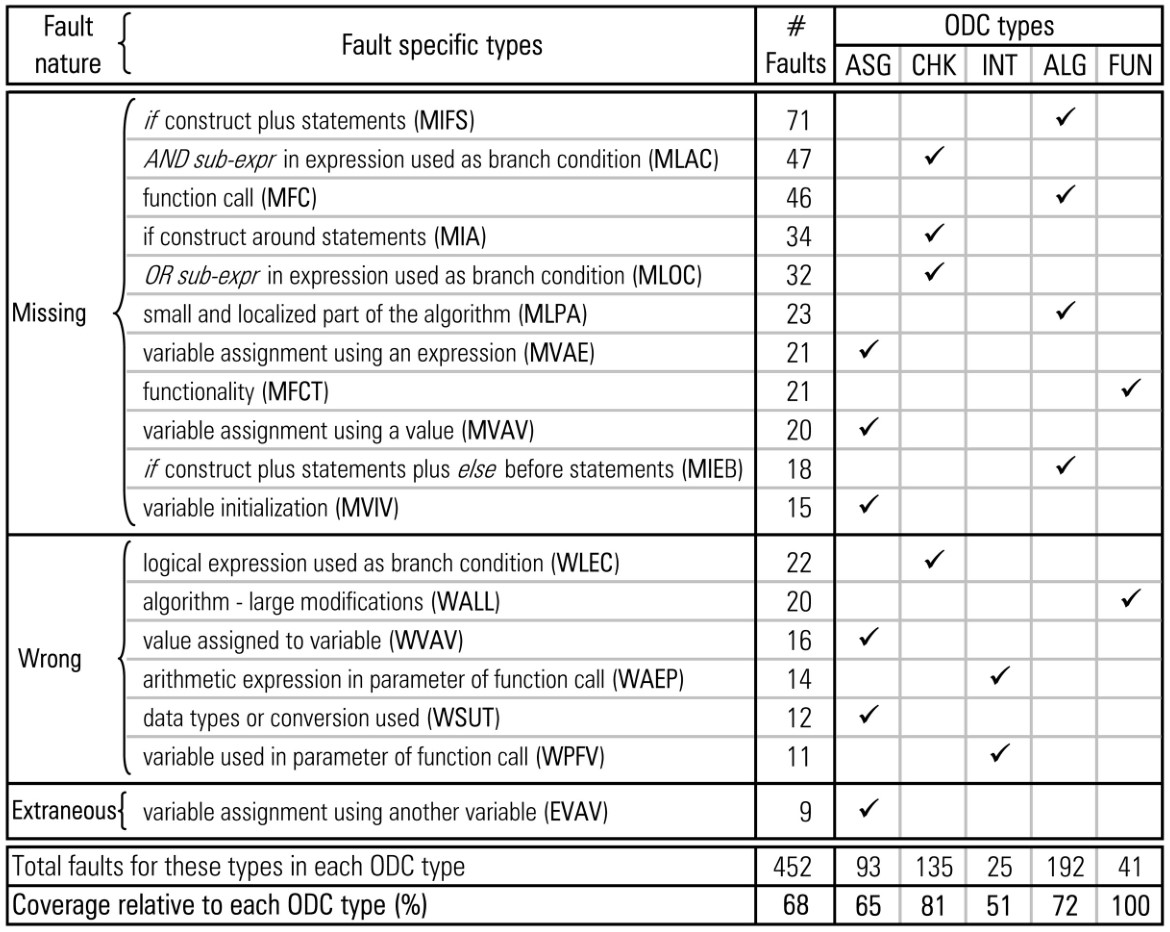
\includegraphics[width=1\textwidth]{img/representative_faults.jpg}
\end{tabular}
\caption{\small \sl Representativeness faults.\label{tab:representative_faults}}
\end{table}

\subsection{Generate derivations}

I chose to use the most representative faults \cite{duraes2006emulation}, divided into missing, wrong and extraneous, specified individually further down:

\red{Table of more representative faults of Durães}

\subsubsection{Fault Types - Missing:}
\begin{itemize}
	\item \textbf{MIFS} - if construct plus statements

	This operator is based in the remotion of one conditional if. To do that, I need to verify the constraints c02, c08 and c09.
	\item \textbf{MLAC} - AND sub-expression in expression used as branch condition
	\item \textbf{MFC}  - function call
	\item \textbf{MIA}  - if construct around statements
	\item \textbf{MLOC} - OR sub-expression in expression used as branch condition
	\item \textbf{MLPA} - small and localized part of the algorithm
	\item \textbf{MVAE} - variable assignment using an expression
	\item \textbf{MFCT} - functionality
	\item \textbf{MVAV} - variable assignment using an value
	\item \textbf{MIEB} - if construct plus statements plus else before statements
	\item \textbf{MVIV} - variable initialization
\end{itemize}

\subsubsection{Fault Types - Wrong:}
\begin{itemize}
	\item \textbf{WLEC} - logical expression used as branch condition
	\item \textbf{WALL} - algorithm - large modifications
	\item \textbf{WVAV} - value assigned to variable
	\item \textbf{WAEP} - arithmetic expression in parameter of function call
	\item \textbf{WSUT} - data types or conversion used
	\item \textbf{WPFV} - variable used in parameter of function call
\end{itemize}

\subsubsection{Fault Types - Extraneous:}
\begin{itemize}
	\item \textbf{EVAV} - variable assignment using another variable
\end{itemize}

\subsection{Constraints}

The constraints defined below was specified by João Durães in ... .

\begin{table}[ht]
\centering
\begin{tabular}{|c|l|}
\hline
\textbf{Constraints}            & \multicolumn{1}{c|}{\textbf{Description}}                                     \\ \hline \hline
\textbf{C01}       \label{C01}  & Return value of the function \textbf{must not} being used                              \\ \hline
\textbf{C02}       \label{C02}  & Call \textbf{must not be} the only statement in the block                              \\ \hline
\textbf{C03}       \label{C03}  & Variable \textbf{must be} inside stack frame                                           \\ \hline
\textbf{C04}       \label{C04}  & \textbf{Must be} the first assignment for that variable in the module                  \\ \hline
\textbf{C05}       \label{C05}  & Assignment \textbf{must not be} inside a loop                                          \\ \hline
\textbf{C06}       \label{C06}  & Assignment \textbf{must not be} part of a for construct                                \\ \hline
\textbf{C07}       \label{C07}  & \textbf{Must not be} the first assignment for that variable in the module              \\ \hline
\textbf{C08}       \label{C08}  & The if construct \textbf{must not be} associated to an else construct                  \\ \hline
\textbf{C09}       \label{C09}  & Statements \textbf{must not include more than} five statements and not include loops   \\ \hline
\textbf{C10}       \label{C010} & Statements are in the same block, \textbf{do not include more than} 5 stats. not loops \\ \hline
\textbf{C11}       \label{C011} & There \textbf{must be} at least two variables in this module                           \\ \hline
\end{tabular}
\end{table}

\newpage
\section{Work plan and implications}

Built three separated modules:

\begin{itemize}
	\item Generate the derivations of main code of selected programs;
	\item Verify and analyze the effect of produced faults;
	\item Compile the programs with injected faults, by using make file.
\end{itemize}

\subsection{Analyze the effects}

The fault injected results is equal to the real software faults?

\subsection{Compile programs}

\red{Select five to ten programs to test.}

After the compilation and execution of the programs, the results need to be evaluate. For that, I will use the \textit{CRASH Scale}\cite{koopman1997comparing}:

\begin{itemize}
	\item \textbf{C}atastrophic
	\item \textbf{R}estart
	\item \textbf{A}bort
	\item \textbf{S}ilent
	\item \textbf{H}indering
\end{itemize}